\documentclass[12pt,a4paper,ngerman]{article}
\usepackage{stylesheet}
\usepackage{epstopdf}

\begin{document}
\TUHeader                          %  Bitte Ausfüllen!!!
%----------------------------
{Digitale Übertragungssysteme}                       %  Übungstitel
%----------------------------
{28.10.2014}                        %  Übungsdatum
%----------------------------
{05}                            %  Gruppen-Nr.
%----------------------------
{Thomas Pichler}                   % Name des Protokollführers
%----------------------------
{
1.~Daniel Freßl, 1230028\\
2.~Thomas Neff, 1230319\\                    %  Übungsteilnehmer
3.~Thomas Pichler, 1230320 \\                   %  ...bei <4 Teilnehmer auskommentieren
4.~Martin Winter, 1130688\\
}
%----------------------------
{Assoc.-Prof. Dipl.-Ing. Dr. Klaus Witrisal}
{Katharina Ritt}                          %  Betreuer
%----------------------------
{Graz}                              %  Ort der Protokollerstellung
{\today}                            %  Datum Protokollerstellung




\pagebreak
  
\tableofcontents
  
\pagebreak

%-------------------------------------------------------------------------------
%
% Beginn des Protokolls
%
%-------------------------------------------------------------------------------

\section{Aufgabe 1}
\subsection{Aufgabenstellung}
In dieser Aufgabe sollen mit Hilfe des BERTool die Bitfehlerkurven von Q-PSK und 8-PSK ermittelt werden. \\
Die erhaltenen Bitfehlerkurven sollen diskutiert werden. \\

\subsection{Schaltung}
Es wurde keine Schaltung benötigt.

\subsection{Formeln}
Es wurden keine Formeln benötigt.

\subsection{Berechnungsbeispiele}
Es wurden keine Berechnungen durchgeführt.
\pagebreak
\subsection{Diagramme}
\begin{figure}[h!]
\centering
\includegraphics[scale=0.4]{figures/1_QPSK_8PSK_BER.png} 
\caption{Bit error rate für QPSK und 8-PSK in Abhängigkeit von $\frac{E_b}{N_0}$}
	\label{fig:qpsk_8psk_ber}
	\end{figure}
	
\pagebreak	

\subsection{Geräteliste}
PC mit BERTool

\subsection{Diskussion}
Bei dieser Aufgabe wurden mit dem BERTool die theoretischen Bitfehlerkurven für QPSK und 8-PSK geplottet. \\
Die dafür notwendigen Einstellungen waren: \\

\begin{table}[h!]
\begin{center}
\begin{tabular}{ |c|c| }

  \hline
  $\frac{E_b}{N_0}$ range: & 0:18 dB \\
  \hline
  Channel type: & AWGN \\ \hline
  Modulation type: & PSK \\ \hline
  Modulation order: & 4 für QPSK oder 8 für 8-PSK \\ \hline
  Channel coding: & None \\
  \hline
\end{tabular}
\caption{Einstellungen im BERTool}
\label{tab:BERTool}
\end{center}
\end{table}


Im Diagramm (Figure 1) ist die Bitfehlerwahrscheinlichkeit über dem Signal-Rausch-Verhältnis pro Bit für QPSK und 8-PSK aufgetragen. \\
Die Kurve für QPSK liegt unter der Kurve für 8-PSK. Daraus kann man ablesen, dass bei gleichen Signal-Rausch-Verhältnis die Bitfehlerwahrscheinlichkeit bei QPSK geringer ist oder man bei gleicher Fehlerwahrscheinlichkeit ein geringeres $\frac{E_b}{N_0}$ benötigt. \\
Dies ist damit zu erklären, dass die Symbole (im I/Q-Diagramm) bei QPSK einen größeren euklidischen Abstand zueinander haben als bei 8-PSK. Somit ist 8-PSK im Vergleich zu QPSK störanfälliger. \\
Am Ende der Aufgabe wurden noch weitere Bitfehlerkurven für verschiedene Kanäle und Modulationen geplottet und diskutiert.




\pagebreak
\section{Aufgabe 2}
\subsection{Aufgabenstellung}
Ziel dieser Aufgabe ist es, mit einem Versuchsaufbau die zuvor am Modell gewonnenen Erkenntnisse praktisch zu verifizieren. Mit dem Übungsaufbau soll ein Übertragungssystem mit einem Satellitenmodem simuliert werden. \\
Es werden Daten vom Bit Error Analyzer erzeugt, diese werden mittels digitaler Schnittstelle an das Satelliten-Modem übertragen. Das Satelliten-Modem codiert und moduliert diese Daten ($2048$ kbit/s) und gibt sie als Signal im Zwischenfrequenzband (ZF = $70$ MHz) aus. Dieses Signal wird am Kanal mit Hilfe eines Rauschgenerators gestört und am Spektrum-Analysator untersucht. Gleichzeitig werden die gesendeten Daten wieder vom Empfangszweig des Modems aufgenommen und demoduliert sowie dekodiert und das Ergebnis über die digitale Schnittstelle zurück an den Bit Error Analyzer übermittelt. \\
Folgende Schritte sind nun mit Hilfe des Versuchsaufbaus durchzuführen:

\begin{enumerate}
\item Bestimmen Sie die Bitfehlerkurven für QPSK-Modulation mit $R_c = \frac{7}{8}$, 8PSK-Modulation mit $R_c = \frac{7}{8}$ und 8-PSK-Modulation mit $R_c = \frac{3}{4}$.
\item Ermitteln Sie die 3dB-HF-Bandbreite des Signals.
\item Diskussion der Bandbreiteneffizienz verschiedener Modulationsarten. Warum stimmen praktische und theoretische Kurven nicht ganz überein?
\item Der Codiergewinn bei einer vorgegebenen Bitfehlerwahrscheinlichkeit zwischen den beiden verwendeten 8PSK-Modulationen ist zu ermitteln und zu diskutieren! Was geschieht mit der Bandbreite? Was geschieht mit der Datenrate?
\end{enumerate}





\subsection{Schaltung}
\begin{figure}[h!]
\centering
\includegraphics[scale=0.6]{figures/2_schaltung.png} 
\caption{Schaltung zur Messung der BER bei verschiedenen Codierungsverfahren und Modulationsverfahren. Schaltung aus \emph{Digitale Modulation}\cite[S.25]{2_schematic}}
	\label{fig:qpsk_8psk_ber}
	\end{figure}
	
\subsection{Tabellen}

\begin{center}
\begin{table}[h!]


\centering
\begin{tabular}{ |c|c|c|c|c|c| }
  \hline
    & Power level & $\frac{S+N}{N}$ & BER & $\frac{S}{N}$ & $\frac{E_b}{N_0}$\\
  \hline
  Einheit & dB & dB & - & dB & dB \\
  \hline
  Messung 1 & $-11$ & $11$ & $1$ & $10.6406$ & $4.0535$ \\
  \hline
    Messung 2 & $-10$ & $12$ & $5.69\cdot10^{-2}$ & $11.717$ & $4.4636$ \\
  \hline
    Messung 3 & $-9$ & $13$ & $3.57\cdot10^{-2}$ & $12.7767$ & $4.8673$ \\
  \hline
    Messung 4 & $-8$ & $14$ & $9.34\cdot10^{-5}$ & $13.8236$ & $5.2661$ \\
  \hline
    Messung 5 & $-7$ & $15$ & $0$ & $14.8604$ & $5.6611$ \\
  \hline
    Messung 6 & $-6$ & $16$ & $0$ & $15.8895$ & $6.0531$ \\
  \hline    
\end{tabular}
\caption{Messung von SNR, BER und $\frac{E_b}{N_0}$ bei 8PSK mit $R_c = \frac{7}{8}$.\label{tab:8psk_7_8}}
\end{table}

\end{center}

\begin{center}
\begin{table}[h!]
\centering


\begin{tabular}{ |c|c|c|c|c|c| }
  \hline
    & Power level & $\frac{S+N}{N}$ & BER & $\frac{S}{N}$ & $\frac{E_b}{N_0}$\\
  \hline
  Einheit & dB & dB & - & dB & dB \\
  \hline
  Messung 1 & $-6$ & $15$ & $0$ & $14.8604$ & $8.4917$ \\
  \hline
    Messung 2 & $-7$ & $14$ & $0$ & $13.8236$ & $7.8992$ \\
  \hline
    Messung 3 & $-8$ & $13$ & $0$ & $12.7767$ & $7.3010$ \\
  \hline
    Messung 4 & $-9$ & $12$ & $0$ & $11.717$ & $6.6954$ \\
  \hline
    Messung 5 & $-9.5$ & $11.5$ & $0$ & $11.1811$ & $6.3892$ \\
  \hline
    Messung 6 & $-10$ & $11$ & $1$ & $10.6406$ & $6.0803$ \\
  \hline    
\end{tabular}
\caption{Messung von SNR, BER und $\frac{E_b}{N_0}$ bei QPSK mit $R_c = \frac{7}{8}$.\label{tab:qpsk_7_8}}
\end{table}

\end{center}

\begin{center}
\begin{table}[h!]

\centering

\begin{tabular}{ |c|c|c|c|c|c| }
  \hline
    & Power level & $\frac{S+N}{N}$ & BER & $\frac{S}{N}$ & $\frac{E_b}{N_0}$\\
  \hline
  Einheit & dB & dB & - & dB & dB \\
  \hline
  Messung 1 & $-10$ & $12$ & $1$ & $11.717$ & $5.2075$ \\
  \hline
    Messung 2 & $-9.5$ & $12.5$ & $1$ & $12.2486$ & $5.4438$ \\
  \hline
    Messung 3 & $-9$ & $13$ & $5.3\cdot10^{-3}$ & $12.7767$ & $5.6785$ \\
  \hline
    Messung 4 & $-8.5$ & $13.5$ & $5.3\cdot10^{-5}$ & $13.3015$ & $5.9118$ \\
  \hline
    Messung 5 & $-8$ & $14$ & $5.61\cdot10^{-7}$ & $13.8236$ & $6.1438$ \\
  \hline
    Messung 6 & $-7$ & $15$ & $0$ & $14.8604$ & $6.6046$ \\
  \hline    
\end{tabular}
\caption{Messung von SNR, BER und $\frac{E_b}{N_0}$ bei 8PSK mit $R_c = \frac{3}{4}$.\label{tab:qpsk_7_8}}
\end{table}

\end{center}
\pagebreak
\subsection{Formeln}

Berechnung des SNR:
\begin{equation}\label{eq:snr_db}
 \frac{S}{N}_{[dB]} = 10 \cdot log_{10}(10^{(\frac{S+N}{N}_{[dB]})} -1) 
\end{equation}


Berechnung der Symbolrate:
\begin{equation}\label{eq:rs_formula}
 r_s = \frac{r_b}{log_2(M) \cdot R_c}
\end{equation}

Die Nyquistbandbreite ist im HF-Bereich gleich der Symbolrate. Die äquivalente Rauschbandbreite $B_R$ ist, dadurch, dass wir einen Raised-Cosine-Filter verwenden, gleich der Nyquistbandbreite.
\begin{equation}\label{eq:bn_rs_formula}
 B_R = B_N = r_s
\end{equation}

Berechnung der erhöhten Bandbreite durch Raised-Cosine-Filter
\begin{equation}
 B = B_N \cdot (1 + \alpha)
\end{equation}

Das SNR pro bit $\frac{E_b}{N_0}_{[dB]}$ hängt ab vom SNR, der äquivalenten Rauschbandbreite $B_R$ und der Bitrate $r_b$.
\begin{equation}
 \frac{E_b}{N_0}_{[dB]} = \frac{S}{N}_{[dB]} \cdot \frac{B_R}{r_b} 
\end{equation}



\subsection{Berechnungsbeispiele}

Berechnungsbeispiele aus Tabelle \ref{tab:8psk_7_8}, Messung 1:

Gegebene Größen: $r_b = 2048 kbit/s$, $R_c = \frac{7}{8}$, $M = 8$, $\alpha = 1$

\begin{equation}
 \frac{S}{N}_{[dB]} = 10 \cdot log_{10}(10^{(\frac{S+N}{N}_{[dB]})} -1) =  10 \cdot log_{10}(10^{11} -1) = 10.6406 dB
\end{equation}

\begin{equation}
 r_s = \frac{r_b}{log_2(M) \cdot R_c} = \frac{2048 kbit/s}{log_2(8) \cdot \frac{7}{8}} = 780190.47 s^{-1}
\end{equation}

\begin{equation}\label{eq:bn_8psk_7_8}
 B_R = B_N = r_s = 780190.47 Hz
\end{equation}

\begin{equation}
 B = B_N \cdot (1 + \alpha) = 780190.47 Hz \cdot (1 + 1) = 1560380.95 Hz
\end{equation}

\begin{equation}
 \frac{E_b}{N_0}_{[dB]} = \frac{S}{N}_{[dB]} \cdot \frac{B_R}{r_b} = 10.6406 \cdot \frac{780190.47 Hz}{2048 kbit/s} = 4.0535 dB
\end{equation}

Berechnung der benötigten Bandbreite für QPSK ($M = 4$) mit $R_c = \frac{7}{8}$

\begin{equation}
 r_s = \frac{r_b}{log_2(M) \cdot R_c} = \frac{2048 kbit/s}{log_2(4) \cdot \frac{7}{8}} = 1170285.7 s^{-1}
\end{equation}

\begin{equation}\label{eq:bn_qpsk_7_8}
 B_N = r_s = 1170285.7 Hz
\end{equation}

\begin{equation}
 B = B_N \cdot (1 + \alpha) = 780190.47 Hz \cdot (1 + 1) = 2340571.43 Hz
\end{equation}

Berechnung der benötigten Bandbreite für 8PSK ($M = 8$) mit $R_c = \frac{3}{4}$

\begin{equation}
 r_s = \frac{r_b}{log_2(M) \cdot R_c} = \frac{2048 kbit/s}{log_2(8) \cdot \frac{3}{4}} = 910222.22 s^{-1}
\end{equation}

\begin{equation}\label{eq:bn_8psk_3_4}
 B_N = r_s = 910222.22 Hz
\end{equation}

\begin{equation}
 B = B_N \cdot (1 + \alpha) = 780190.47 Hz \cdot (1 + 1) = 1820444.44 Hz
\end{equation}
\pagebreak
\subsection{Diagramme}
\begin{figure}[h!]
\hspace*{-3cm}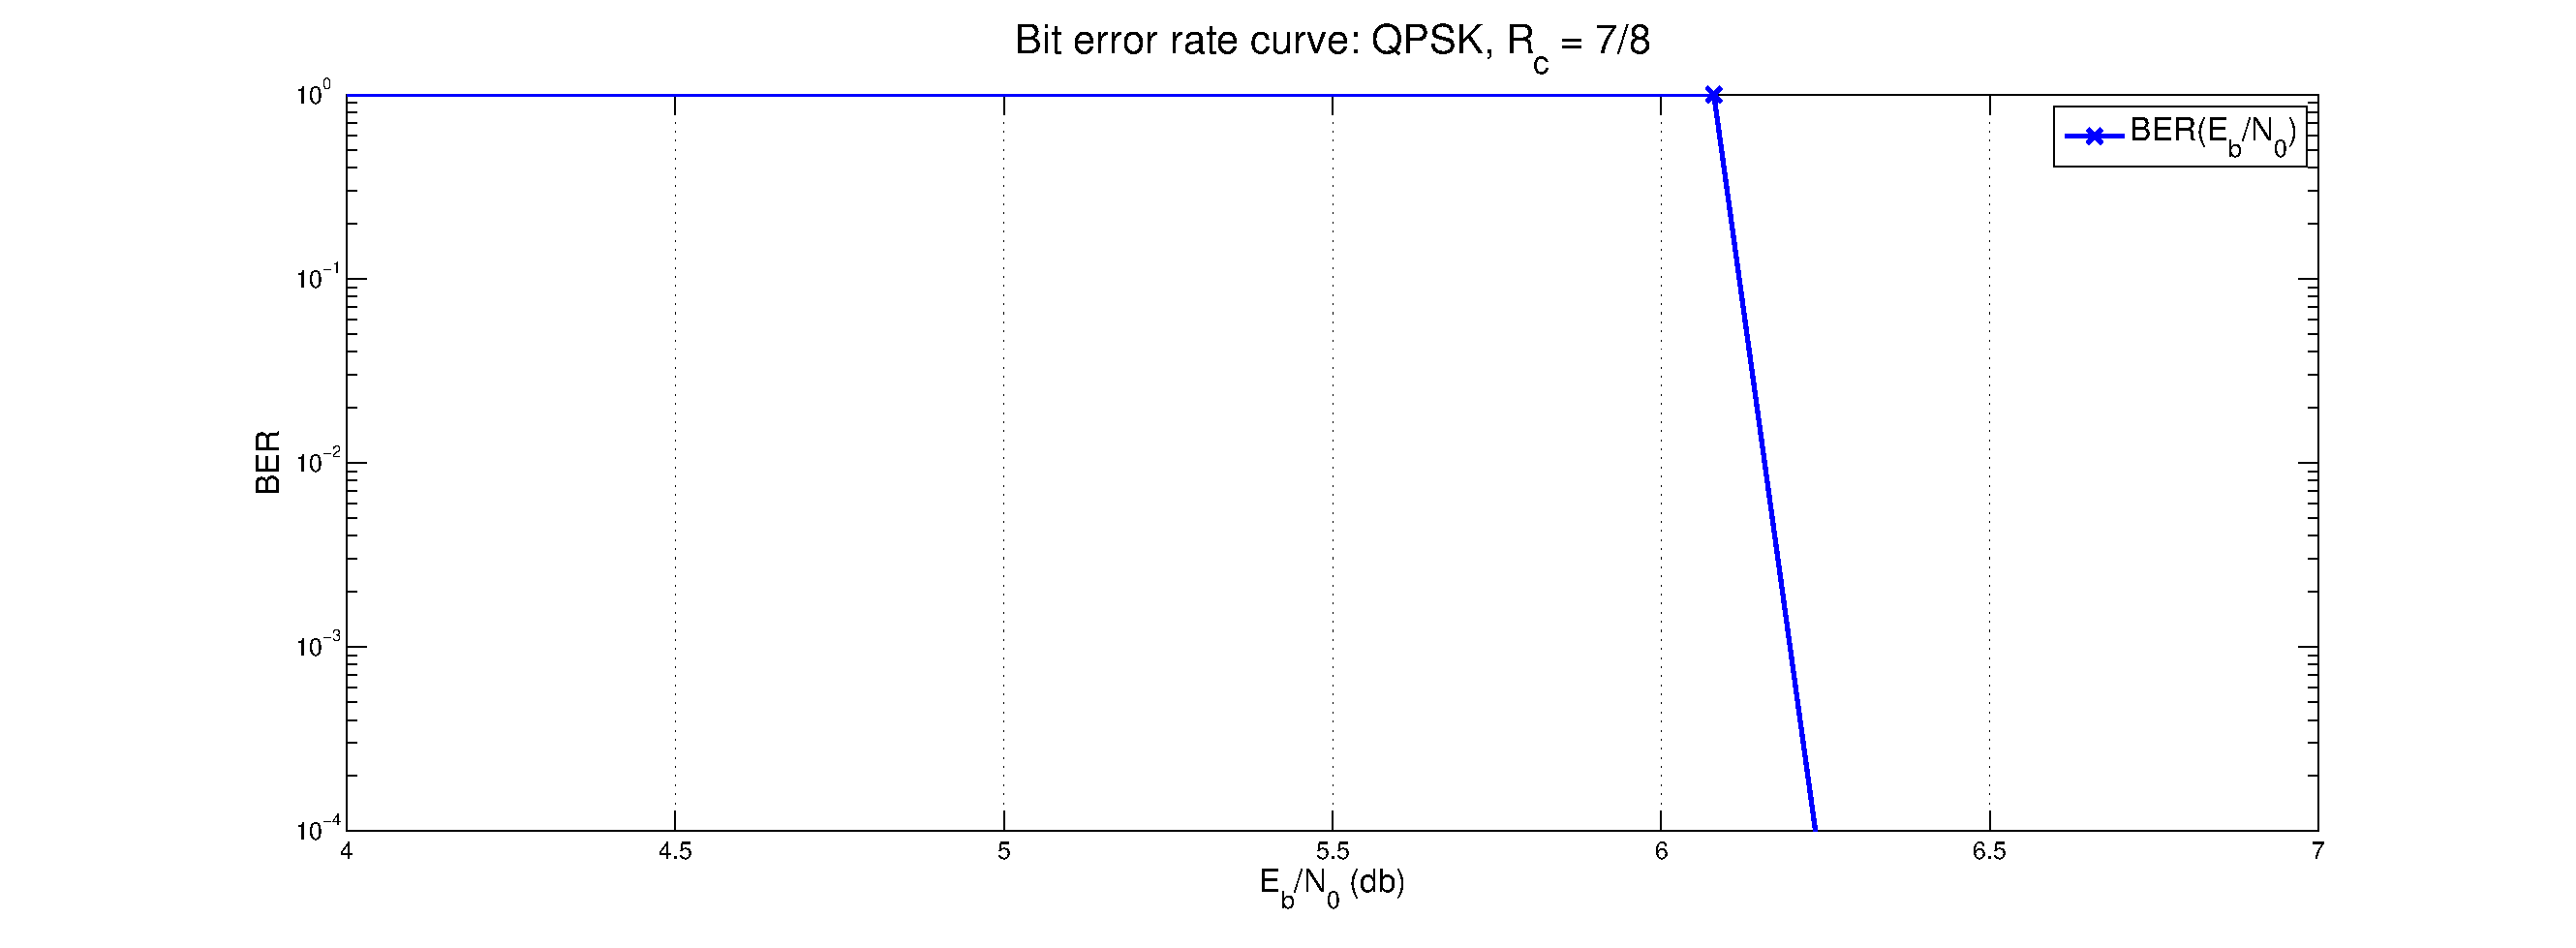
\includegraphics[scale=0.5]{figures/qpsk_ber_eb_n0.eps} 
\caption{BER für QPSK mit $R_c = \frac{7}{8}$ in Abhängigkeit von $\frac{E_b}{N_0}$}
	\label{fig:ber_qpsk}
	\end{figure}
	
	\begin{figure}[h!]
\hspace*{-3cm}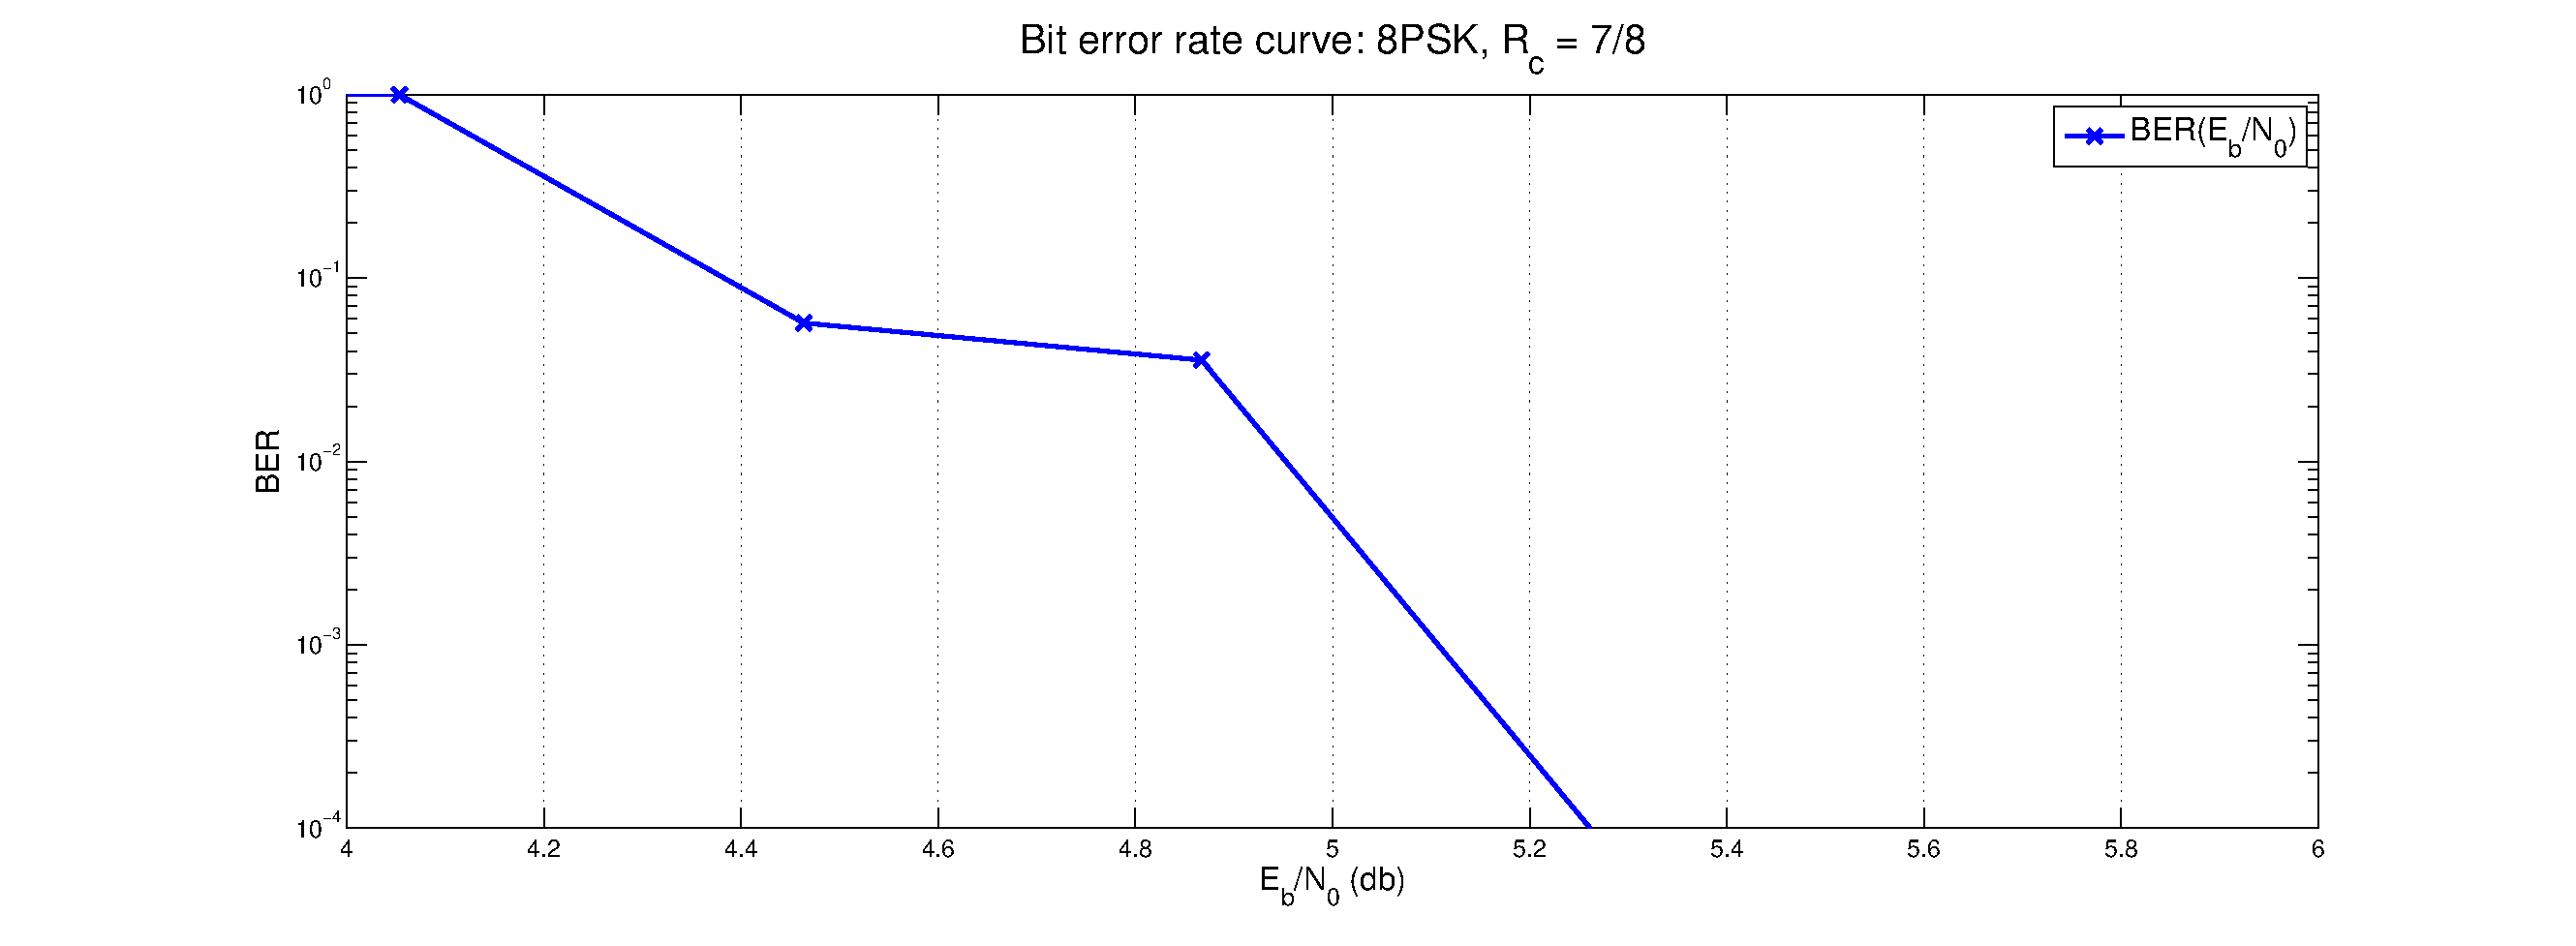
\includegraphics[scale=0.5]{figures/8psk_ber_eb_n0.eps} 
\caption{BER für 8PSK mit $R_c = \frac{7}{8}$  in Abhängigkeit von $\frac{E_b}{N_0}$}
	\label{fig:ber_8psk}
	\end{figure}
	\pagebreak
	\begin{figure}[h!]
\hspace*{-3cm}\includegraphics[scale=0.5]{figures/8psk_ber_eb_n0_3_4.eps} 
\caption{BER für 8PSK mit $R_c = \frac{3}{4}$  in Abhängigkeit von $\frac{E_b}{N_0}$}
	\label{fig:ber_8psk_3_4}
	\end{figure}
	
		\begin{figure}[h!]
\hspace*{-3cm}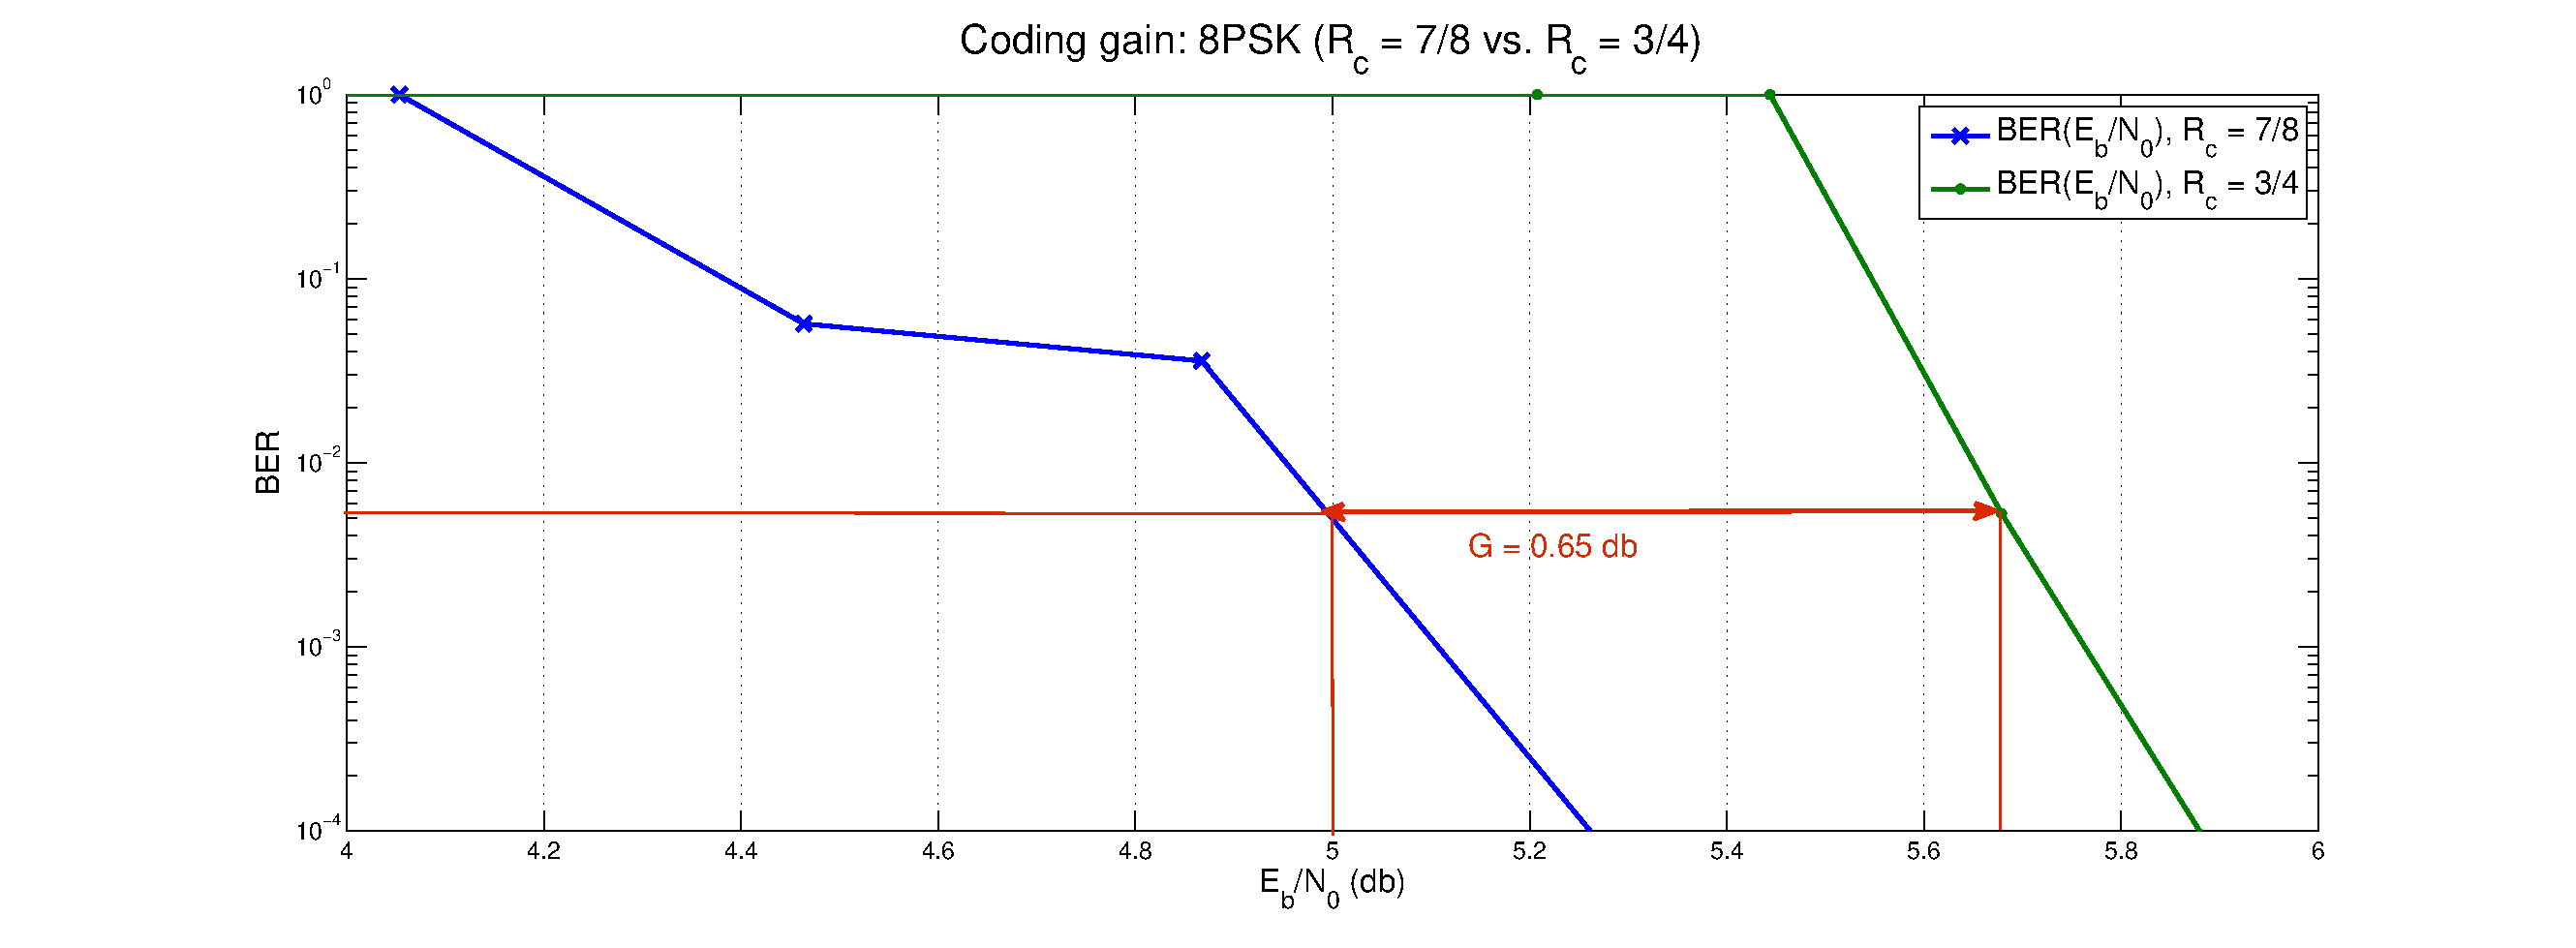
\includegraphics[scale=0.5]{figures/8psk_coding_gain.eps} 
\caption{Codiergewinn für 8PSK bei $BER = 5\cdot10^{-3}$ für $R_c = \frac{3}{4}$ und $R_c = \frac{7}{8}$}
	\label{fig:8psk_coding_gain}
	\end{figure}
	\pagebreak
	
\begin{figure}[h!]
\includegraphics[scale=0.5]{figures/spec_ana.png} 
\caption{Anzeige des Spektrum-Analyzers und Messung des Signal-Rauschleistungsverhältnisses bei Übung 2}
	\label{fig:spec_ana}
	\end{figure}	
	
	\pagebreak
	\pagebreak

\subsection{Geräteliste}

\begin{center}
\begin{table}[h!]
\centering

\begin{tabular}{ |l|l| }
  \hline
  Name & Inventarnummer \\
  \hline
  Network Analyzer (Rohde \& Schwarz 9kHz - 3GHz) & 0144481 \\ \hline
  Satellitenmodem (Radyne ComStream DMD20) & 0119641 \\ \hline
  Digital Communicatios Analyzer PFA-30 & 0051709 \\ \hline
  Rauschgenerator & - \\ \hline
  PC & - \\
  \hline
\end{tabular}
\caption{Geräteliste Aufgabe 2.\label{tab:geraeteliste2}}
\end{table}
\end{center}
	
	\clearpage
\subsection{Diskussion}
Bei dieser Aufgabe wurden einige Messungen mithilfe eines Satellitenmodems, eines Spektrum-Analyzers und eines Bit-Error-Generators durchgeführt.

Die Messung des Signal-Rauschleistungsverhältnis lässt sich anhand der Darstellung des Spektrum-Analyzers erklären.

Wie in Abbildung \ref{fig:spec_ana} eingezeichnet, wird zuerst das Verhältnis $\frac{S+N}{N}$ gemessen, in dem die Differenz zwischen maximaler und minimaler Amplitude des Spektrums gebildet wird.

Für große $\frac{S+N}{N}$ ($>20dB$) lässt sich das Signal-Rauschleistungsverhältnis gut als $\frac{S+N}{N} = \frac{S}{N}$ annähern. Für kleinere $\frac{S+N}{N}$ muss das Signal-Rauschleistungsverhältnis anhand Formel \ref{eq:snr_db} berechnet werden. 

Zu Aufgabe 2: Die 3dB-HF-Bandbreite ist gleich der Nyquistbandbreite im Bandpassbereich. Diese Bandbreite ist wiederum gleich der Symbolrate. (siehe Formel \ref{eq:rs_formula})

In die Berechnung der Symbolrate fließen folgende Faktoren mit ein: Die Anzahl der Symbole $M$, die übertragen werden können, die Informationsbitrate $r_b$ und die Coderate $R_c$.

Die Ergebnisse der 3dB-HF-Bandbreite für die verwendeten Modulationsverfahren und Codierungen liefern Formel \ref{eq:bn_qpsk_7_8}, Formel \ref{eq:bn_8psk_3_4} und Formel \ref{eq:bn_8psk_7_8}.

Man sieht, dass bei gleichbleibender Datenrate 8PSK deutlich weniger Bandbreite benötigt als QPSK. Außerdem ist zu erwähnen, dass 8PSK mit $R_c = \frac{7}{8}$ sowohl weniger Bandbreite benötigt, als auch eine bessere Bitfehlerkurve besitzt als 8PSK mit $R_c = \frac{3}{4}$.
(Siehe Abbildung \ref{fig:ber_8psk}, Abbildung \ref{fig:ber_8psk_3_4} und Abbildung \ref{fig:8psk_coding_gain})

Bei unseren Messungen war es uns außerdem nicht möglich, genauere Daten für QPSK aufzunehmen, da bei der geringsten möglichen Änderung der Signalleistung sich die Bitfehlerrate von 0\% auf 100\% geändert hat.

Da die Coderate von $R_c = \frac{3}{4}$ eigentlich eine bessere Bitfehlerkurve besitzen sollte, sind hier anscheinend Ungenauigkeiten bei der Messung aufgetreten.


Bei Übung 1 wurden die theoretischen Verläufe von diversen Modulations- und Codierungsverfahren analysiert. Diese weichen jedoch von den praktischen Kurven ab. Das lässt sich dadurch erklären, dass das Übertragungssystem nicht angepasst war und die Filter nicht beliebig genau sind. 

Zu Punkt 4: Wir haben den Codiergewinn zwischen 8PSK mit $R_c = \frac{3}{4}$ und 8PSK mit $R_c = \frac{7}{8}$ bei einer Bitfehlerrate von $0.5\%$ betrachtet. Mit unseren Messergebnissen ergibt sich hier ein Codiergewinn von $G = 0.65 dB$. Die Datenrate ist bei unseren Messungen immer konstant geblieben, allerdings verändert sich durch die verschiedenen Coderaten die benötigte Bandbreite. (Änderung der Coderate bedeutet Änderung der gesendeten Redundanz-Bits, damit auch Änderung der benötigten Bandbreite.)





\pagebreak



\section{Aufgabe 3}
\subsection{Aufgabenstellung}
Ziel dieser Aufgabe ist es die zuvor verwendeten Modulationsverfahren einer detaillierteren Betrachtung zu unterziehen. Es sollen dazu mittels einer  MatLab-Simulationsumgebung BPSK, QPSK, 8-PSK und 16-QAM im Basisband bei unterschiedlichen Roll-Off-Faktoren und SNR-Werten untersucht werden. \\
Dabei werden vor allem der Bandbreitenbedarf anhand des Spektrums sowie der Einfluss durch Rauschen anhand des Spektrums, Augendiagramms und Phasenstern des jeweiligen Modulationsverfahrens genauer diskutiert. Diese MatLab-Simulation ist so normiert, dass von einer Kanalbitrate von 1 bit/s ausgegangen wird, dahier ist die äquivalente Nyquist-Bandbreite im Basisband genau 0.5 Hz. \\
\begin{enumerate}
\item Ermitteln Sie für BPSK die Auswirkung des Roll-Off-Faktors auf die Bandbreite? Zu welcher Erkenntnis kommen Sie? Warum bleibt das SNR trotz größerer Filterbandbreite konstant?

\item Womit ist die Veränderung des Augendiagramms für unterschiedliches $\alpha$ erklärbar?
\item Ermitteln Sie den Bandbreitenbedarf für unterschiedliche Modulationsverfahren (BPSK, QPSK, 8-PSK,16-QAM) für ein beliebig gewähltes $\alpha$ und SNR.
\item Vergleichen Sie das Augendiagramm von BPSK und QPSK ($\alpha$ und SNR konstant). Was können Sie erknnen und wie begründen sie es?
\item Vergleichen Sie das Augendiagramm von BPSK und 8-PSK ($\alpha$ und SNR konstant). Was können Sie erknnen und wie begründen sie es?
\item Vergleichen Sie das Augendiagramm von 8-PSK und 16-QAM ($\alpha$ und SNR konstant). Was können Sie erknnen und wie begründen sie es?
\item  Ermitteln Sie den Einfluss von ansteigendem Rauschen (Verringerung des SNR) auf unterschiedliche Modulationsverfahren. Hinweis: Ermitteln Sie für jedes Modulationsverfahren den ungefähren SNR-Wert, bei welchem eine augenscheinlich fehlerfreie Detektion (Demodulation) nicht mehr bzw. gerade noch möglich ist. Vergleichen Sie die Ergebnisse der unterschiedlichen Modulationsverfahren. Was schließen Sie daraus? 
\end{enumerate}

\pagebreak
	
\pagebreak
\clearpage
\subsection{Tabellen}
\begin{center}
\begin{table}[h!]
\centering

\begin{tabular}{ |l|l|l| }
  \hline
  & $\alpha$ & B \\
  \hline
  Einheit & - & Hz \\ \hline
  & 0 & 1 \\ \hline
  & 0.1 & 1.1 \\ \hline
  & 0.2 & 1.2 \\ \hline
  & 0.3 & 1.3 \\ \hline
  & 0.4 & 1.36 \\ \hline
  & 0.5 & 1.46 \\ \hline
  & 0.6 & 1.54 \\ \hline
  & 0.7 & 1.6 \\ \hline
  & 0.8 & 1.72 \\ \hline
  & 0.9 & 1.8 \\ \hline
  & 1 & 1.95 \\
  \hline
\end{tabular}
\caption{Verschiedene $\alpha$-Werte bei konstantem SNR (50dB).\label{tab:TABcossweep}}
\end{table}
\end{center}
\begin{table}[h!]
\centering
\begin{tabular}{ |l|l|l| }
  \hline
  & Modulation & B \\
  \hline
  Einheit & - & Hz \\ \hline
  & BPSK & 1 \\ \hline
  & QPSK & 0.5 \\ \hline
  & 8-PSK & 0.32 \\ \hline
  & 16-QAM & 0.24 \\ \hline
  \hline
\end{tabular}
\caption{Bandbreitenbedarf verschiedener Modulationsverfahren.\label{tab:TABmodverf}}
\end{table}

\begin{table}[h!]
\centering
\begin{tabular}{ |l|l|l| }
  \hline
  & Modulation & B \\
  \hline
  Einheit & - & Hz \\
  \hline
  & BPSK & 10 \\ \hline
  & QPSK & 11 \\ \hline
  & 8-PSK & 19 \\ \hline
  & 16-QAM & 18 \\ 
  \hline
\end{tabular}
\caption{Maximales SNR bei verschiedenen Modulationsverfahren.\label{tab:TABmaxsnr}}
\end{table}


\pagebreak


\subsection{Schaltung}
Es wurde keine Schaltung benötigt.

\subsection{Formeln}
Es wurde keine Formeln benötigt.

\subsection{Berechnungsbeispiele}
Es wurden keine Berechnungen durchgeführt.

\subsection{Diagramme}


\begin{figure}[h!]
\centering
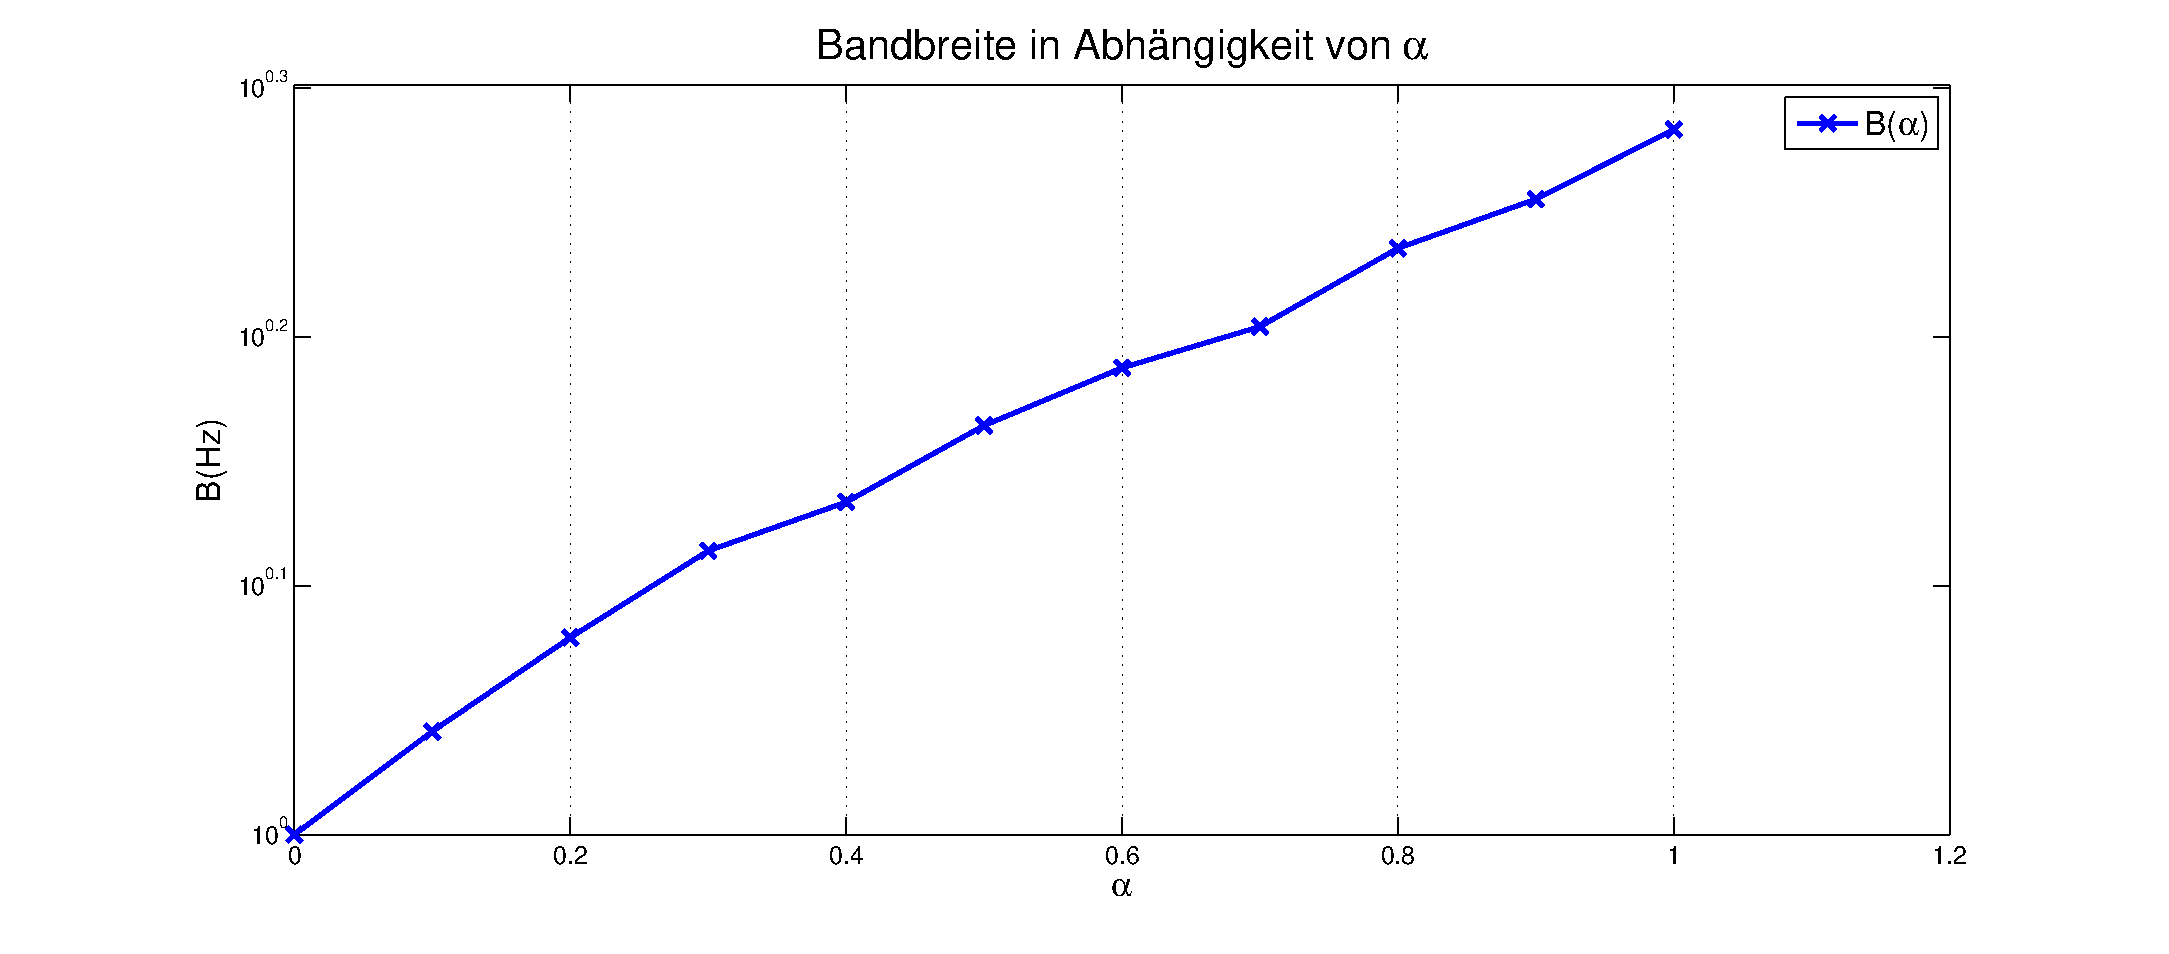
\includegraphics[scale=0.4]{figures/3_B(alpha).eps} 
\caption{Bandbreite B in Abhängigkeit von $\alpha$}
\label{fig:3_B}
\end{figure}

\begin{figure}[h!]
\centering
\includegraphics[scale=0.4]{figures/3a_1.png} 
\caption{Auswirkung des Roll-Off-Faktors auf die Bandbreite $\alpha=0$}
\label{fig:3_A_1}
\end{figure}

\begin{figure}[h!]	
\centering
\includegraphics[scale=0.4]{figures/3a_2.png} 
\caption{Auswirkung des Roll-Off-Faktors auf die Bandbreite $\alpha=1$}
\label{fig:3_A_2}
\end{figure}
	
\begin{figure}[h!]
\centering
\includegraphics[scale=0.4]{figures/3d_bpsk.png} 
\caption{Augendiagramm von BPSK}
\label{fig:3_C}
\end{figure}
	
\begin{figure}[h!]
\centering
\includegraphics[scale=0.4]{figures/3d_qpsk.png} 
\caption{Augendiagramm von QPSK}
\label{fig:3_D}
\end{figure}
\pagebreak
\pagebreak
	
\clearpage
	
\subsection{Geräteliste}
PC mit MatLab/Simulink	
	
\subsection{Diskussion}
Zu Punkt 1: Wie aus dem Abbildung \ref{fig:3_B} , bzw. Tabelle \ref{tab:TABcossweep} zu entnehmen ist, steigt die Bandbreite nahezu linear mit dem Roll-Off-Faktor. Somit ist gezeigt worden, dass die Formel $B = B_N\cdot(1+\alpha)$ korrekt ist. Das bedeutet, dass das SNR konstant bleibt, weil die äquivalente Rauschbandbreite bei einem Raised-Cosinus-Filter nur von der Nyquistfrequenz abhängt und diese gleich bleibt.

Zu Punkt 2: Wie aus Abbildung \ref{fig:3_A_1} und Abbildung \ref{fig:3_A_2} deutlich zu erkennen ist, sinkt mit steigendem $\alpha$ die Steilheit des Signales, dafür wird das Augendiagramm schärfer. Die Veränderung des Diagramms kann daher auf das Jittern zurückgeführt werden. Ist $\alpha$ = $0$, so entspricht das der idealen Sincfunktion. Bei $\alpha$ = $1$ ist man flexibler im Abtastpunkt, jeodch ist die Sincfunktion weit entfernt vom Ideal. Damit ergibt sich die Eigenschaft, dass man bei $\alpha$ = $0$ viel genauer abtasten muss, als bei $\alpha$ = $1$.

Zu Punkt 3: Wie aus Tabelle \ref{tab:TABmodverf} zu entnehmen, ergibt sich je nach Modulationsverfahren ein unterschiedlicher Bandbreitenbedarf. Der Bandbreitenbedarf nimmt mit dem Grad der Modulation ab (bei QPSK $\frac{1}{2}$, 8PSK $\frac{1}{3}$ und 16QAM $\frac{1}{4}$ der Bandbreite von BPSK). Was auch nicht anders zu erwarten war, da das der Sinn der verschiedenen Verfahren ist.

Zu Punkt 4: Wie aus den Screenshots (Abbildung \ref{fig:3_C} und Abbildung \ref{fig:3_D}) zu entnehmen ist, gibt es keine Änderung des Augendiagrammes bei BPSK und QPSK. Begründen lässt sich dies dadurch, dass der Abstand der einzelnen Zeichen zueinander, bei beiden Modulationsverfahren, gleich groß ist.

Zu Punkt 5: Das Augendiagramm von 8-PSK hat im Gegensatz zum Augendiagramm von BPSK kleinere Distanzen zwischen den Symbolen. Außerdem gibt es mehr Amplitudenzustände. Dadurch zeigen sich im Augendiagramm nicht zwei, sondern vier Amplitudenstufen am Abtastzeitpunkt. \emph{Leider sind die bei uns in der Laborübung aufgenommenen Screenshots zum Augendiagramm von 8-PSK korrupt, weswegen wir kein Bild in das Protokoll einfügen konnten.}

Zu Punkt 6: Das Augendiagramm von 16-QAM hat im Gegensatz zu QPSK mehr Amplitudenzustände, sowie unterschiedliche Abstände zwischen den Symbolen. Das Augendiagramm sieht also ähnlich aus wie das von 8-PSK, allerdings mit anderen Amplituden der Stufen am Abtastzeitpunkt.\emph{Leider sind die bei uns in der Laborübung aufgenommenen Screenshots zum Augendiagramm von 16-QAM korrupt, weswegen wir kein Bild in das Protokoll einfügen konnten.}\\

Für das SNR bei den Punkten 4 bis 6 wurde 50dB und für $\alpha$ 0 gewählt.\\

\pagebreak

Zu Punkt 7: Wie aus Tabelle \ref{tab:TABmaxsnr} zu entnehmen ist, sind die SNR-Werte bei QPSK und BPSK ungefähr gleich. Der Grund liegt an der Anordnung um den Einheitskreis. Da die euklidischen Abstände gleich sind, ist auch der Störabstand gleich und somit auch das SNR. Bei 8-PSK und 16QAM sind die euklidischen Abstände zwischen den Symbolen ebenfalls ähnlich groß. Daher ist das SNR ungefähr gleich groß. Die euklidischen Abstände von 8PSK/QAM sind im Vergleich zu BPSK/QPSK kleiner. Deshalb ist die Störfestigkeit geringer und man benötigt ein höheres SNR für die Übertragung.  Gewonnene Erkenntnis: Umso geringer die Euklid'sche Distanz, umso mehr SNR benötigt man. 




 \begin{thebibliography}{9}

\bibitem{2_schematic}
  Dipl.-Ing. Eral Türkyilmaz,
  \emph{Digitale Modulation},
  Technische Universität Graz,
  Version 1.1, 2014,

\end{thebibliography}



   
\end{document}

